\documentclass{beamer}
\usepackage{epstopdf}
\usepackage{tabularx}
\usepackage{adjustbox}
\usepackage{pdflscape}
\usepackage[]{hyperref}
\definecolor{links}{HTML}{0B610B} % dark green
%\definecolor{links}{HTML}{2A1B81} % dark blue
\hypersetup{colorlinks,linkcolor=,urlcolor=links}
\usepackage{multirow} % for tables
\usepackage{multicol}
\usepackage{subfig}
\usepackage{graphicx}
\usetheme{Madrid}
\title[Hashing classification for tracking ]{Hashing Classification for charged particle tracking}
\author[Luiza Adelina Ciucu (ATLAS) ]{Luiza Adelina Ciucu (ATLAS)} 

\titlegraphic{
%
\includegraphics[height=2.1cm]{./physics_section_EN_q.eps} 

\includegraphics[height=2.1cm]{./physics_section_EN_q-eps-converted-to.pdf} 
}

\date{22 May 2020}

\begin{document}

\frame{\titlepage}

%\texttt{\detokenize{

% define input folder for our plots only once
\newcommand\inputFolderMerged{../output_new_ev_000_030}
\newcommand\inputFolderOverlay{../output_overlay_balanced_ev_000_030}


% add some useful definitions
%\def\MeV{\ifmmode {\mathrm{\ Me\kern -0.1em V}}\else
%                   \textrm{Me\kern -0.1em V}\fi}%  

\def\volumeID{\texttt{\detokenize{volume_id}}}
\def\layerID{\texttt{\detokenize{layer_id}}}

\def\TP{\ifmmode {\mathrm{TP}}\else
                   \textrm{TP}\fi}%
\def\FP{\ifmmode {\mathrm{FP}}\else
                   \textrm{FP}\fi}%                                     
\def\FN{\ifmmode {\mathrm{FN}}\else
                   \textrm{FN}\fi}%
\def\TN{\ifmmode {\mathrm{TN}}\else
                   \textrm{TN}\fi}%

% intro slide
\begin{frame}{Introduction}
\begin{enumerate}
\item[o] Compare two methods to balance the number of positive and negative hits : unbalanced (A) and balanced (B).
\item[o] Used 30 events. Each group of 10: 7 in train, 3 in test. 
\item[o] Unbalanced (A): keep all buckets (with default weight of 1.0).
\item[o] Balanced (B): remove buckets so that bucket distribution is symmetric around 10 in NbPositiveHit per bucket (with default weight of 1.0).
\item[o] Used min 0, 4, 7 and 10 positive hits in the bucket; if less, consider all hits in the bucket to be negative, but use same reweighting as above.
\item[o] How a bucket is created:
\begin{enumerate}
\item[-] Loop over events, and for each event build annoy index and then:
\item[-] Loop over hits and for each hit build a bucket using annoy and 20 nearest neighbours by direction
\item[-] Loop over hits in the bucket, find their particleID; find particleID with most hits in the bucket; denote it majority particle.
\item[-] Loop over hits in the bucket again, if belongs to the majority particle assign output +1, else -1.
\end{enumerate}
\end{enumerate}
\end{frame}
\clearpage

\begin{frame}{Histogram NbBuckets vs NbPositiveHit in a bucket}
\begin{enumerate}
\item[o] \textcolor{red}{Unbalanced} (\textcolor{blue}{Balanced})  \textcolor{red}{are not} (\textcolor{blue}{are}) symmetric around 10. 
\end{enumerate}
\centering
% plots
\includegraphics[width=0.48\textwidth]{\inputFolderMerged/plot_histo_2_NbBucket_vs_NbPositiveHit_Train.pdf}
\includegraphics[width=0.48\textwidth]{\inputFolderMerged/plot_histo_2_NbBucket_vs_NbPositiveHit_Test.pdf}\\
\includegraphics[width=0.48\textwidth]{\inputFolderMerged/plot_histo_2_NbBucket_vs_NbPositiveHit_normalized_Train.pdf}
\includegraphics[width=0.48\textwidth]{\inputFolderMerged/plot_histo_2_NbBucket_vs_NbPositiveHit_normalized_Test.pdf}\\
\end{frame}

\begin{frame}{Count buckets in each NbPositiveHit category.}
\begin{enumerate}
\item[o] Balanced around 10 NbPositiveHit via bucket removal.
\item[o] 0 and 1 no buckets $\rightarrow$ 19 and 20 are balanced to no buckets (ignored). 
\end{enumerate}
\centering
% plots
\includegraphics[width=0.8\textheight]{\inputFolderMerged/Balanced_30_buckets.png}
\end{frame}

\begin{frame}{OutputPositive and PredictedOutputPositive 1/2}
\begin{enumerate}
\item[o] Min00 (left) and Min04 (right)
\end{enumerate}
\centering
% plots
\includegraphics[width=0.43\textwidth]{\inputFolderOverlay_Min00/plot_02_1_overlay_histo_OutputPositive_Test.pdf}
\includegraphics[width=0.43\textwidth]{\inputFolderOverlay_Min04/plot_02_1_overlay_histo_OutputPositive_Test.pdf}\\
\includegraphics[width=0.43\textwidth]{\inputFolderOverlay_Min00/plot_02_1_overlay_histo_PredictedOutputPositive_Test.pdf}
\includegraphics[width=0.43\textwidth]{\inputFolderOverlay_Min04/plot_02_1_overlay_histo_PredictedOutputPositive_Test.pdf}\\
\end{frame}


\begin{frame}{OutputPositive and PredictedOutputPositive 2/2}
\begin{enumerate}
\item[o] Min07 (left) and Min10 (right).
\item[o] Min10 and method Unbalanced predicts all hits to be negative.
\end{enumerate}
\centering
% plots
\includegraphics[width=0.43\textwidth]{\inputFolderOverlay_Min07/plot_02_1_overlay_histo_OutputPositive_Test.pdf}
\includegraphics[width=0.43\textwidth]{\inputFolderOverlay_Min10/plot_02_1_overlay_histo_OutputPositive_Test.pdf}\\
\includegraphics[width=0.43\textwidth]{\inputFolderOverlay_Min07/plot_02_1_overlay_histo_PredictedOutputPositive_Test.pdf}
\includegraphics[width=0.43\textwidth]{\inputFolderOverlay_Min10/plot_02_1_overlay_histo_PredictedOutputPositive_Test.pdf}\\
\end{frame}

\begin{frame}{Metrics for each VolumeID overlay two methods 1/2.}
\begin{enumerate}
\item[o] Min00 and Min04 very similar. 
\end{enumerate}
\centering
% table
\begin{center}
\begin{tabular}{ |c|c|c| } 
\hline
Accuracy & Precision & Recall \\ 
\hline
$\frac{\TP+\TN}{\TP+\FP+\FN+\TN}$ & $\frac{\TP}{\TP+\FP}$  & $\frac{\TP}{\TP+\FN}$ \\ 
\hline
\end{tabular}
\end{center}
% plots
\includegraphics[width=0.32\textwidth]{\inputFolderOverlay_Min00/plot_03_1_overlay_graph_Accuracy_VolumeID_Test.pdf}
\includegraphics[width=0.32\textwidth]{\inputFolderOverlay_Min00/plot_03_1_overlay_graph_Precision_VolumeID_Test.pdf}
\includegraphics[width=0.32\textwidth]{\inputFolderOverlay_Min00/plot_03_1_overlay_graph_Recall_VolumeID_Test.pdf}\\
\includegraphics[width=0.32\textwidth]{\inputFolderOverlay_Min04/plot_03_1_overlay_graph_Accuracy_VolumeID_Test.pdf}
\includegraphics[width=0.32\textwidth]{\inputFolderOverlay_Min04/plot_03_1_overlay_graph_Precision_VolumeID_Test.pdf}
\includegraphics[width=0.32\textwidth]{\inputFolderOverlay_Min04/plot_03_1_overlay_graph_Recall_VolumeID_Test.pdf}\\
\end{frame}

\begin{frame}{Metrics for each VolumeID overlay two methods 2/2.}
\begin{enumerate}
\item[o] \item[o] Min10 learns all hits to be negative, so precision and recall at zero.
\end{enumerate}
\centering
% table
\begin{center}
\begin{tabular}{ |c|c|c| } 
\hline
Accuracy & Precision & Recall \\ 
\hline
$\frac{\TP+\TN}{\TP+\FP+\FN+\TN}$ & $\frac{\TP}{\TP+\FP}$  & $\frac{\TP}{\TP+\FN}$ \\ 
\hline
\end{tabular}
\end{center}
% plots
\includegraphics[width=0.32\textwidth]{\inputFolderOverlay_Min07/plot_03_1_overlay_graph_Accuracy_VolumeID_Test.pdf}
\includegraphics[width=0.32\textwidth]{\inputFolderOverlay_Min07/plot_03_1_overlay_graph_Precision_VolumeID_Test.pdf}
\includegraphics[width=0.32\textwidth]{\inputFolderOverlay_Min07/plot_03_1_overlay_graph_Recall_VolumeID_Test.pdf}\\
\includegraphics[width=0.32\textwidth]{\inputFolderOverlay_Min10/plot_03_1_overlay_graph_Accuracy_VolumeID_Test.pdf}
\includegraphics[width=0.32\textwidth]{\inputFolderOverlay_Min10/plot_03_1_overlay_graph_Precision_VolumeID_Test.pdf}
\includegraphics[width=0.32\textwidth]{\inputFolderOverlay_Min10/plot_03_1_overlay_graph_Recall_VolumeID_Test.pdf}\\
\end{frame}


\begin{frame}{Metrics for each VolumeID with min value used.}
\begin{enumerate}
\item[o] Min00 and Min04 very similar. 
\item[o] Min10 learns all hits to be negative, so precision and recall at zero.
\end{enumerate}
\centering
% table
\begin{center}
\begin{tabular}{ |c|c|c| } 
\hline
Accuracy & Precision & Recall \\ 
\hline
$\frac{\TP+\TN}{\TP+\FP+\FN+\TN}$ & $\frac{\TP}{\TP+\FP}$  & $\frac{\TP}{\TP+\FN}$ \\ 
\hline
\end{tabular}
\end{center}
% plots
\includegraphics[width=0.32\textwidth]{\inputFolderOverlay_Unbalanced/plot_03_1_overlay_graph_Accuracy_VolumeID_Test.pdf}
\includegraphics[width=0.32\textwidth]{\inputFolderOverlay_Unbalanced/plot_03_1_overlay_graph_Precision_VolumeID_Test.pdf}
\includegraphics[width=0.32\textwidth]{\inputFolderOverlay_Unbalanced/plot_03_1_overlay_graph_Recall_VolumeID_Test.pdf}\\
\includegraphics[width=0.32\textwidth]{\inputFolderOverlay_Balanced/plot_03_1_overlay_graph_Accuracy_VolumeID_Test.pdf}
\includegraphics[width=0.32\textwidth]{\inputFolderOverlay_Balanced/plot_03_1_overlay_graph_Precision_VolumeID_Test.pdf}
\includegraphics[width=0.32\textwidth]{\inputFolderOverlay_Balanced/plot_03_1_overlay_graph_Recall_VolumeID_Test.pdf}\\
\end{frame}

\begin{frame}{Conclusion. Future plans.}
\begin{enumerate}
\item[o] Conclusions:
  \begin{enumerate}
\item[-] Compared two methods: Unbalanced vs Balanced.
\item[-] Balanced: remove buckets such that number of buckets with a given nbPositiveHit is symmetric around 10.
\item[-] 0 and 1 no buckets $\rightarrow$ 19 and 20 are balanced to no buckets (ignored). 
\item[-] For each Unbalanced and Balanced, did Min00, Min04, Min07, Min10.
\item[-] As seen before, Unbalanced Min10 learns all hits to be negative, so precision and recall are zero.
\item[-] Min00 and Min04 are very similar.
\item[-] Min07 in between Min04 and Min10.
\item[-] \textbf{Overall, balancing buckets improve performance.}
\end{enumerate}
\item[o] Future plans:
\begin{enumerate}
\item[-] Balance buckets in majority particle $\eta$. Is it replacing the balancing of nbPositiveHit, or in addition to it?
\end{enumerate}
\end{enumerate}
\end{frame}

\end{document}

\begin{frame}{Conclusion. Future plans.}
\begin{enumerate}
\item[o] Conclusions:
\begin{enumerate}
\item[-] Compared two methods: Unbalanced vs Balanced.
\item[-]
\item[-]
\end{enumerate}
\item[o] Future plans:
\begin{enumerate}
\item[-]
\item[-]
\item[-]
\end{enumerate}
\end{enumerate}
\end{frame}

\end{document}
